\chapter[Lecture 18]{}\label{lec18}

{\bf Force Constant :} Effective forces in metals are quite long-range and are carried from ion to ion by conduction electrons.

The range can be as long as 20 planes!

Assume, we need $p$ planes for the dispersion relation
$$
\therefore\quad w^{2}=\dfrac{2}{M}\sum\limits_{k>0}C_{p}(1-\cos pka)
$$
Multiply both sides by $\cos nka$ and integrate over independent range of $k\to$
\begin{align*}
M\int\limits^{\pi/a}_{-\pi/a}d_{k}w^{2}_{k}\cos nka &= 2\sum\limits_{k>0}C_{p}\int\limits^{\pi/a}_{-\pi/a}dk(1-\cos pka)\cos nka\\
&= 2\pi \dfrac{C_{n}}{a}
\end{align*}
integral vanishes except $p=n$.
$$
\therefore\quad \fbox{$C_{p}=-\dfrac{Ma}{2\pi}\int\limits^{\pi/a}_{-\pi/a}dk w^{2}_{k}\cos pka$}
$$
$C_{p}$ is the force constant at range $pa$, for a structure with monatonic basis.

\section*{Crystal with a Basis}

Phonon dispersion shows new features in the presence of a basis.

Lets assume, there are two atoms in the basis; like NaCl crystal.

For convenience, consider direction of propagation such that the planes contain one kind of atom. [111] - direction 
\begin{figure}[H]
\centering
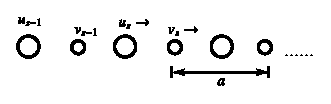
\includegraphics[scale=1.5]{images/lecture18/fig1.eps}
\end{figure}
The equation of motion will be
\begin{align*}
M_{1}\dfrac{d^{2}u_{s}}{dt^{2}} &= C(v_{s}+v_{s-1}-2u_{s})\\
M_{2}\dfrac{dv_{s}}{dt^{2}} &= C(u_{s+1}+u_{s}-2v_{s})
\end{align*}
The trial solution can be
$$
u_{s}=u\exp (iska) \exp (-iwt)\quad v_{s}=v\exp (iska)\exp(-iwt)
$$
On substitution, we get
\begin{equation*}
\left.
\begin{array}{l}
-w^{2}M_{1}u = Cv[1+\exp(-ika)]-2Cu\\
-w^{2}M_{2}v=Cu[\exp(ika)+1]-2Cv
\end{array}\right]\tag{A}\label{lec18-eqA}
\end{equation*}

This will have a solution for $u$ and $v$ if the determinant vanishes.
$$
w^{4}-2C\left(\frac{1}{M}+\frac{1}{M_{2}}\right)w^{2}+\dfrac{e^{2}k^{2}a^{2}}{M_{1}M_{2}}=0
$$
\begin{align*}
\Rightarrow \ w^{2} &= C\left(\dfrac{1}{M_{1}}+\dfrac{1}{M_{2}}\right)\pm \sqrt{C^{2}\left(\frac{1}{M_{1}}+\frac{1}{M_{2}}\right)^{2}-\dfrac{C^{2}k^{2}a^{2}}{M_{1}M_{2}}}\\
&= C\left(\dfrac{1}{M_{1}}+\dfrac{1}{M_{2}}\right)\pm C\sqrt{\left(\frac{1}{M_{1}}+\frac{1}{M_{2}}\right)^{2}-\dfrac{k^{2}a^{2}}{M_{1}M_{2}}}\\
&= C\left(\frac{1}{M_{1}}+\frac{1}{M_{2}}\right)\pm C\left(\dfrac{1}{M_{1}}+\frac{1}{M_{2}}\right)\left[1+\frac{k^{2}a^{2}M_{1}M_{2}}{(M_{1}+M_{2})^{2}}\right]^{\frac{1}{2}}\\
&= 2C\left(\frac{1}{M_{1}}+\frac{1}{M_{2}}\right)\quad\text{and}\quad \frac{1}{2}\cdot C\left(\frac{1}{M_{1}}+\frac{1}{M_{2}}\right)\frac{k^{2}a^{2}M_{1}M_{2}}{(M_{1}+M_{2})^{2}}=\frac{\frac{1}{2}C}{M_{1}+M_{2}}\cdot k^{2}a^{2}
\end{align*}
\begin{gather*}
\left|
\begin{array}{lc}
2C-M_{1}w^{2} & -C[1+\exp(-ika)]\\
-C[1+\exp(ika)] & 2C-M_{2}w^{2}
\end{array}
\right|=0
\tag{B}\label{lec18-eqB}\\
\Rightarrow\quad (2C-M_{1}w^{2})(2C-M_{2}w^{2})-C^{2}(2+\exp(-ika)+\exp(ika))=0\\
a, \fbox{$M_{1}M_{2}w^{4}-2C(M_{1}+M_{2})w^{2}+2C^{2})(1-\cos ka)=0$}\tag{lec18-eqC}
\end{gather*}
This equation can be solved exactly for $w^{2}$.

However let's look at the limiting cases.

For $ka\ll 1$ and $ka=\pm \pi$

For $ka\ll 1$\quad $1-\cos ka=2\sin^{2}\dfrac{ka}{2}\simeq \frac{1}{2}k^{2}a^{2}$
\begin{equation*}
\therefore\quad \fbox{$w^{2}\simeq 2C\left(\frac{1}{M_{1}}+\frac{1}{M_{2}}\right)$}\quad\text{and}\quad \fbox{$\dfrac{\frac{1}{2}C}{M_{1}+M_{2}}k^{2}a^{2}$}\tag{lec18-eqD}
\end{equation*}
For $ka=\pm \dfrac{\pi}{a}$
\begin{equation*}
\fbox{$w^{2}=\dfrac{2C}{M_{1}}$ and $\dfrac{2C}{M_{2}}$}\tag{E}\label{lec18-eqE}
\end{equation*}

Lets investigate particle displacements at $k=0$. Substituting the solution of $w^{2}$ for $ka\ll 1$ in \eqref{lec18-eqA} we get.
$$
\dfrac{u}{v}=-\dfrac{M_{2}}{M_{1}}\quad \text{for}\quad w^{2}=2C\left(\frac{1}{M_{1}}+\dfrac{1}{M_{2}}\right)
$$
The atoms vibrate against each other keeping the center of mass fixed.
\begin{figure}[H]
\centering
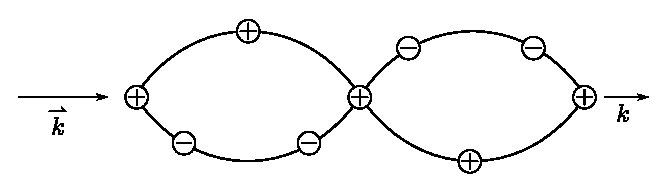
\includegraphics{images/lecture18/fig3.eps}
\end{figure}

Here the motion is similar to the oscillation of an electric field in a light wave $\to$ {\em Optical Branch}.

The second solution gives $u=v$ at $k\neq 0$ limit.
\begin{figure}[H]
\centering
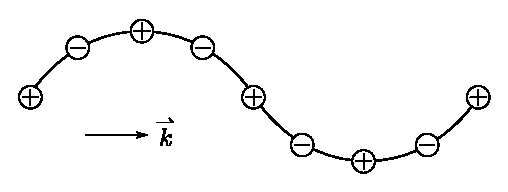
\includegraphics{images/lecture18/fig4.eps}
\end{figure}

Here, the atoms move together like an assoustive wave $\to$ {\em Acoustical branch}.

At the zone boundary, there is a frequency gap between $\sqrt{\dfrac{2C}{M_{1}}}$ and $\sqrt{\dfrac{2C}{M_{2}}}$. This is characteristic feature of elastic waves in poly atomic lattices.
\begin{figure}[H]
\centering
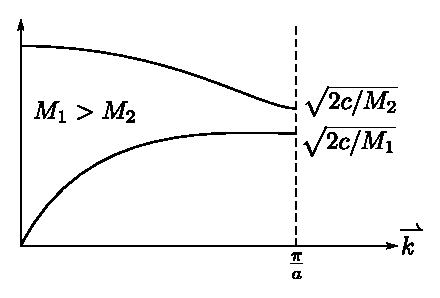
\includegraphics{images/lecture18/fig5.eps}
\end{figure}

For a 3D solid with $N$ cells and $P$ atoms in each primitive cell (basis) $\Rightarrow$ total degrees of freedom $=3pN$.

No. of $k$ values in first Brillouin zone $=N$.

$\therefore \ LA+TA$ modes $=3N$ (one time $LA$ and two times $TA$)

$\therefore \ $ No. of optical modes $=(3P-3)N$

$\therefore \ $ For $P$ atoms in the basis - total $3p$ branches.
$$
3\to \text{Accoustic branches}\quad (3p-3) \to \text{optical branches.}
$$

\section*{Quantization of elastic waves}

Consider an one dimension lattice consisting of $N$ atoms. If $Q_{s}$ represent the position coordinate of $5^{\text{th}}$ atom, For simplicity we can make a boundary condition (closed)
$$
\fbox{$Q_{s}=Q_{s+N}$} \Rightarrow \text{Born-Karman condition type}
$$

$\therefore \ $ The total Hamiltonian of the system will be
\begin{figure}[H]
\centering
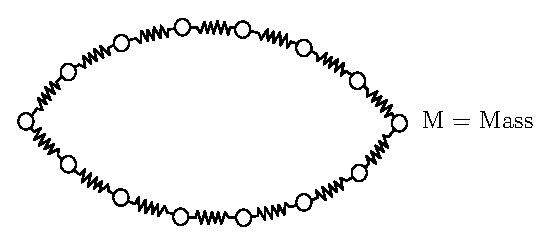
\includegraphics{images/lecture18/fig6.eps}
\end{figure}
$$
H=\sum\limits^{N}_{S=1}\left[\frac{1}{2M}p^{2}_{S}+\frac{1}{2}C(Q_{S+1}-Q_{S})^{2}\right]
$$
assuming harmonic approximation. One can disentangle this Hamiltonian, using normal coordinate system.
\begin{align*}
Q_{S} &= \frac{1}{\sqrt{N}}\sum\limits_{k}Q_{k}e^{iksa}\\[2pt]
Q_{k} &= \frac{1}{\sqrt{N}}\sum\limits_{s}Q_{S}e^{-iksa}\\[2pt]
k &= \frac{2\pi n}{Na}\quad n=0, \pm 1, \pm 2\cdot \pm \left(\dfrac{N}{2}-1\right), \dfrac{N}{2}\\[2pt]
p_{S} &= \frac{1}{\sqrt{N}}\sum\limits_{k}P_{k}e^{-iksa}\\[2pt]
P_{k} &= \dfrac{1}{\sqrt{N}}\sum\limits_{S}p_{s}e^{iksa}
\end{align*}
{\bf N.B.} Exponentials are not same in the FT of $Q_{s}$ and $p_{s}$

Commutation relation $[Q_{r},p_{s}]=i\hbar \delta_{rs} \leftarrow$ Kronecker delta.
\begin{align*}
[Q_{k},P_{k'}] &= \frac{1}{N}\cdot \sum\limits_{r}Q_{r}e^{-ikra}, \sum\limits_{s}p_{s}e^{ik'sa}\\[2pt]
&= \frac{1}{N}\sum\limits_{rs}[Q_{r},p_{s}]e^{-i(kr-k's)a}\leftarrow [q_{r},p_{s}]=i\hbar \delta_{rs}\\[2pt]
&= \frac{2\hbar}{N}\sum\limits_{r}e^{-i(k-k')ra}
\end{align*}
$\therefore \ $ \fbox{$[Q_{k},P_{k'}]=i\hbar \delta_{kk'}$}
\begin{align*}
& \sum\limits_{r}e^{-i(k-k')ra}k>\dfrac{2\pi n}{Na}\\[2pt]
&\quad =\sum\limits_{r}e^{-i2\pi(n-n')\dfrac{r}{N}}\\[2pt]
&\quad =N\delta_{n,n'}=N\delta_{k,k'}
\end{align*}
Substituting $p_{s}$ and $q_{s}$ in the Hamiltonian, we get
\begin{align*}
\sum p^{2}_{s} &= \frac{1}{N}\sum\limits_{s}\sum\limits_{k}\sum\limits_{k'}P_{k}P_{k'}e^{-i(k+k')sa}\\[2pt]
&= \sum\limits_{k}\sum\limits_{k'}P_{k}P_{k'}\delta(k+k')=\sum\limits_{R}P_{k}P_{-k}
\end{align*}
\begin{align*}
\sum\limits_{S}(Q_{s+1}-Q_{s})^{2} &= \frac{1}{N}\sum\limits_{s}\sum\limits_{k}\sum\limits_{k'}Q_{k}Q_{k'}e^{iksa}[e^{ika}-1]\cdot e^{ik'sa}[e^{ik'a}-1]\\[2pt]
&=\sum\limits_{k,k'}Q_{k}Q_{k'}(e^{ika}-1)(e^{ik'a}-1)\sum\limits_{s}\frac{1}{N}\cdot e^{i(k+k')sa}\\[2pt]
&= 2\sum\limits_{k}Q_{k}Q_{-k}(1-\cos ka)\\[2pt]
&= \cancel{2}\sum\limits_{k}Q_{k}Q_{-k}\cdot \dfrac{w^{2}_{k}M}{\cancel{2}C} \left[w_{k}=\sqrt{\dfrac{2C}{M}}\sqrt{1-\cos ka}\right]
\end{align*}
as considered classically.
$$
\therefore\quad H=\sum\limits_{k}\left[\frac{1}{2M}P_{k}P_{-k}+\frac{1}{2}Mw^{2}_{k}Q_{k}Q_{-k}\right]
$$
To get the equation of motion -
\begin{gather*}
i\hbar \overdot{Q}_{k}=[Q_{k},H]=i\hbar P_{-k}/M\\
\therefore\quad i\hbar \overddot{Q}_{k}=[\overdot{Q}_{k},H]=\dfrac{1}{M}[P_{-k},H]=-i\hbar w^{2}_{k}Q_{k}\\
\therefore\quad \fbox{$\overddot{Q}_{k}+w^{2}_{k}Q_{k}=0$}\to
\end{gather*}
equation of a Harmonic occillator.

Energy = $\epsilon_{k}=\left(n_{k}+\frac{1}{2}\right)\hbar w_{k}$
$$
\therefore\quad \text{Total energy } U=\sum\limits_{k}(n_{k}+\frac{1}{2})\hbar w_{k}
$$

Therefore, the energy of lattice vibration is quantized and the quantum of energy is called a {\em Phonon} in analogy to photon for electromagnetic wave.
\begin{itemize}
\item[$\to$] $\epsilon_{n}=\left(n+\dfrac{1}{2}\right)\hbar w$ means the mode is excited to quantum no `$n$' $\Rightarrow$ this means, the mode is occupied by `$n$' phonons.

\item[$\to$] $\dfrac{1}{2}\hbar w$ is zero-point energy.

\item[$\to$] Quantization of mean square phonon amplitude means some kind of a standing wave forms in the lattice. If $u$ is the displacement of a volume element from its equillibrium position at $x$,
$$
\fbox{$u=u_{0}\cos kx\cos wt$}
$$
equation of standing wave.
\end{itemize}

Total energy (average) $=\dfrac{1}{2}(K.E)_{avg}+\dfrac{1}{2}(P.E)_{avg}$ in a simple Harmonic Oscillator.
$$
K.E. = \dfrac{1}{2}\rho \left(\dfrac{\rho u}{\rho t}\right)^{2}\rho = \text{mass density}
$$
$\therefore \ $ Volume integral in a crystal of volume $V$ will be,
\begin{align*}
& \int\limits_{x}\frac{1}{2}\rho u^{2}_{0}a^{2},kx \sin^{2}wt\cdot w^{2}dx\quad \text{for all $x$}\\
&\qquad =\dfrac{1}{4}\rho Vw^{2}u^{2}_{0}\sin^{2}wt
\end{align*}
$\therefore \ $ time average of
\begin{align*}
K.E. &= \frac{1}{8}\rho Vw^{2}u^{2}_{0}\\
&= \frac{1}{2}\left(n+\frac{1}{2}\right)\hbar w\\
\therefore\quad \fbox{$u^{2}_{0}=4\left(n+\frac{1}{2}\right)\hbar/\rho Vw$} &= \text{displacement of the n$^{\text{th}}$ mode.}
\end{align*}
{\bf Momentum :} Phonons interact with photon, neutron, electrons etc.
\begin{description}
\item[{*}{*}{*}] It does not have momentum as it involves relative motion of the atoms.

\item[*] For example, in $H_{2}$ molecule, the coordinate $\overrightarrow{r}_{1}-\overrightarrow{r}_{2}$ does not carry momentum but the centre of mass coordinate $\dfrac{1}{2}(r_{1}+r_{2})$ does, this corresponds to $k=0$ mode.
\end{description}
Elastic scattering of a photon in a crystal satisfy the momentum conservation
$$
k'=k+G
$$
$k\to$ wave vector of incident light

\noindent
$k'\to$ scattered light wave vector

\noindent
$G\to$ Reciprocal lattice vector.

For reflection $\Delta k=k-k'=-G$ or \fbox{$\hbar \Delta k=-\hbar G$}, the crystal will experience a recoil with momentum $=-\hbar G$, which is often too small to be considered.

For inelastic scattering, a phonon may get created with wave vector
$$
\therefore\quad \text{momentum conservation } \Rightarrow \fbox{$\overrightarrow{k'}+\overrightarrow{k}=\overrightarrow{k}+\overrightarrow{G}$}
$$
Sign of $\overrightarrow{k}$ will be (-ve) for annihilation of a phonon.

One can use inelastic neutron scattering to determine phonon dispersions. Conservation law.
$$
\fbox{$\overrightarrow{k}+\overrightarrow{G}=\overrightarrow{k}'\pm \overrightarrow{k}$}
$$
$k$, $k'$ are neutron momentum.

(+ve) and (-ve) sign depends on emission or absorption of phonon in the scattering process.

If $M_{n}$ is the mass of neutron, energy conservation can be written as
$$
\fbox{$\dfrac{\hbar{h}^{2}k^{2}}{2M_{n}}=\dfrac{\hbar^{2}k'^{2}}{2M_{n}}\pm \hbar w$}
$$


